\chapter[Concept]{Concept}
\label{ch:concept}
This chapter is devoted to specification and concept of the resulting web application. The application enables creation and management of online courses and interactive solving the exercises. In this chapter, author of the materials would be further called \textit{teacher} and the solver would be called \textit{student}.

    \section{Courses overview}
    \label{sec:exercises}
    Providing the materials for practising agile programming methods is realised in a form of courses. This section contains description of their concept. Concept of a course detail page is illustrated on sketch \ref{fig:course-detail-sketch} \nameref{fig:course-detail-sketch}, its elements are described in detail the following sections.
        
        \begin{figure}[h]
            \centerline{
                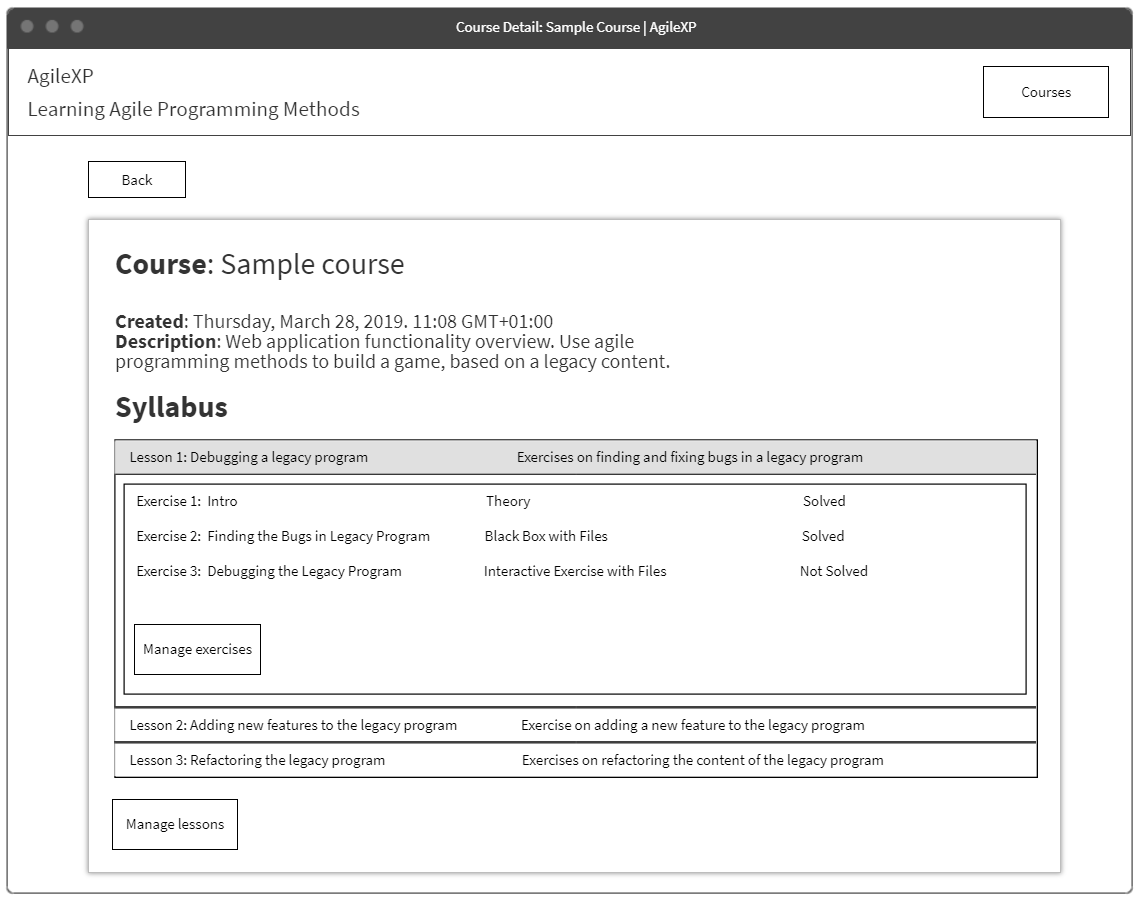
\includegraphics[
                width=0.9\textwidth, width=\linewidth, frame
                ]{images/course-detail-sketch.png}}
            \caption{Course detail sketch}
            \label{fig:course-detail-sketch}
        \end{figure}
        
        \subsection{Courses structure}
        The learning materials have a structure of courses, and each contains lessons with exercises. The course detail page contains a general information for every course element. Application provides tools for creating and editing course elements, they contain a title and description, and lessons and exercises may be reordered. Buttons ``Manage lessons'' ``and Manage exercises'' at course detail page lead to the pages, which provide this functionality. There are five types of exercises, they are specified in detail in section \ref{subsec:exercise-types} \nameref{subsec:exercise-types}. Exercises have different states, depending on progress. Expansion panel is used to show lessons. Each course can be expanded to show the containing exercises. There is an exercise type and progress shown for each.
        
        \subsection{Shown and hidden versions}
        The application provides creation two versions of source code, tests and files. Shown version is shown to the student, when he opens an exercise. Hidden version is not available to him, it is used to running the tests. In most of the exercises, both of the versions are used, but some of them contain only one.
        
        Introducing two versions may be used to show basic code structure to the student, for providing legacy code, or simply for recalling the syntax. On exercise creation, teacher can simply duplicate the hidden version to fill the shown one, but also to create two different.
        
        \subsection{Development environment}
        The web application has convenient development environment, and it is close to conventional IDEs. It consists of code editors with multiple tabs, it is easy to add and remove these tabs. The environment enables code execution and providing a feedback. The application supports use of Java 8 programming language in exercises. Testing framework JUnit 4 is used for testing. As soon as the programming language is Java, the feedback includes not only tests results, but also possible compilation errors. A concept of a code editor is illustrated at sketch \ref{fig:editor-solve-sketch} \nameref{fig:editor-solve-sketch}.
        
        \begin{figure}[h]
            \centerline{
                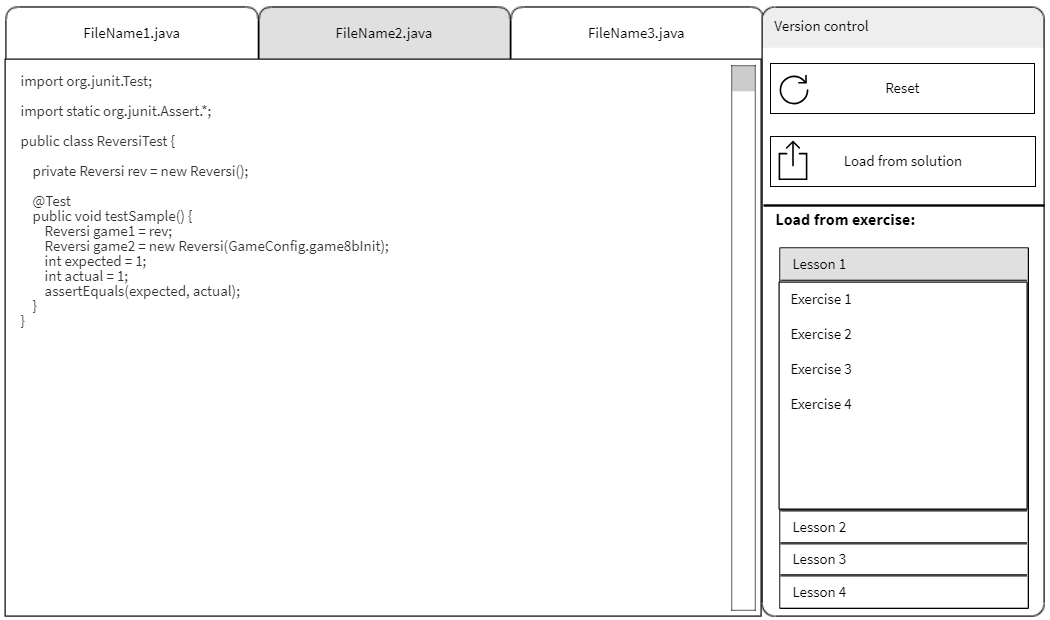
\includegraphics[
                width=0.9\textwidth, width=\linewidth, frame
                ]{images/editor-solve-sketch.png}}
            \caption{Code editor sketch}
            \label{fig:editor-solve-sketch}
        \end{figure}
        
        \subsection{Version control}
        \label{subsec:version-control}
        One of the requirements for the resulting application is version control of the student's solutions. The web application stores and shows source code, tests and files, which are submitted and run by student.
        
        When solving an exercise, the student can view previous versions and copy their files content to the editor. He can access the files from any exercise within a current course. As soon as there is a very large amount of solutions, they all would not be loaded at once, but user may load them page by page. A concept of a version control display is illustrated at sketch of the editor \ref{fig:editor-solve-sketch} \nameref{fig:editor-solve-sketch}.
        
        This feature is useful for refactoring or working with legacy code, e.g. when student needs to extend tests from previous solution with new ones.
        
        \subsection{Solution estimation}
        Solution estimations hold the solution reference and time of its creation. The result is represented with three elements: estimation text, estimation value and a solved flag. Structure of estimation text is different for each exercise type, and is described in section \ref{subsec:exercise-types} \nameref{subsec:exercise-types}. Estimation value is a percentage of progress, and a solved flag tells if it was solved.

        \subsection{Exercise types}
        \label{subsec:exercise-types}
        Environment, which supports only work with source code and estimates solutions automatically, is not enough for practising various agile programming methods. There are five types of exercises to provide different ways of practising agile programming methods separately or in combinations. Their concepts, purpose and usage are described in the following sections.
            
            \subsubsection{Theory}
            Exercise type \textit{Theory} is the basic one, it is aimed to provide information to the student. Such an exercise may be used mainly to introduce or conclude a current course or lesson, or to make an overview on legacy code.
            
            It provides only a text area and is marked as solved at the moment, when is viewed by the student. On exercise creation and update, the teacher can use text editor with ability to format, e.g. to provide example source code. The formatted text is provided to the student.
        
            \subsubsection{Interactive Exercise}
            \label{subsubsec:whitebox}
            \textit{Interactive Exercise} type provides tools for programming.
            On exercise creation, the teacher is required to fill title and description of exercise. Then he uses editors to bring in a shown version of source code. Next editors are designed for tests. Teacher may use them to fill hidden tests to control the solving progress. Also he may provide shown tests, e.g. to recall the JUnit 4 syntax.
            
            On students side, an exercise of this type contains an exercise description and two editors. The first one is for source code, and the second one is for tests. The student may use the environment to solve an exercise, and he may run his code withing the web application and get feedback. The provided feedback consists of two parts. The first one tells about compilation and tests results for the students code from the development environment. The second one is based on the teacher's code, which is not be available for the student.
            
            \subsubsection{Interactive Exercise with Files}
            This exercise type provides the same features as \hyperref[subsubsec:whitebox]{previous one}, and expands its tools with working with files. One more text editor contains files, and there are teachers' and students' versions as well. These files may be used for the purpose of testing.
            
            \subsubsection{Black Box}
            \label{subsubsec:blackbox}
            The next exercise type is named \textit{Black Box}, what means a system or a function, for which only its input and output is known. This term describes the main feature of this type, since the student may not see source code, but may send input and get some form of output from the program. This tool is useful for practising unit testing and test-driven development. On working on this exercise, the student may try to find mistakes in the hidden program with the use of tests.
            
            To create an exercise of this type, teacher should fill its title and description. The second should contain code structure or functions names, or any kind of information to give the student needed knowledge about the hidden code. So he would be able to call necessary functions from his tests. Except filling an exercise title and description on exercise creation, the teacher should enter controlling source code, which would be hidden from the student, it should be compilable and contain several logical mistakes. The application would provide information for the teacher on how to design the source code, so it would be used correctly. The tests, which would be shown to the student, would be filled as well. The purpose of these hidden tests is the same as for such a tests in exercise type \hyperref[subsubsec:whitebox]{\textit{Interactive Exercise}}.
            
            To pass such an exercise, the student should write tests, which would not be passed by the program. The student would run his tests for the hidden program, and would get feedback, telling the number of found mistakes and their total number.
            
            Estimation process was designed in such a way, so only correct solutions can pass. Incorrect solutions are ignored and not counted to the solution. Examples of such a solutions are the following: the student may write test, which would not be passed, but it would not find the mistake. It may happen, if this test would not pass a correct version of the hidden program as well. This solution should be ignored. Another example is writing several tests, so they would find the same mistake several times. Only one test would be counted for solution, the rest would be ignored.
            
            \subsubsection{Black Box with Files}
            This exercise type extends \hyperref[subsubsec:blackbox]{previous one} with ability to work with files, which are used for testing.


    \section{Architecture}
    The application uses client-server architecture, its components are illustrated on \ref{fig:component-diagram} \nameref{fig:component-diagram}.
    
    The topmost presentation level of the application is provided with Browser subsystem. It communicates with Server subsystem, which is responsible for business logic and data access. Server subsystem consists of several components. Server accesses Database server, which belongs to Database subsystem, and am Estimation module.
    
    \begin{sidewaysfigure}
    \centerline{
        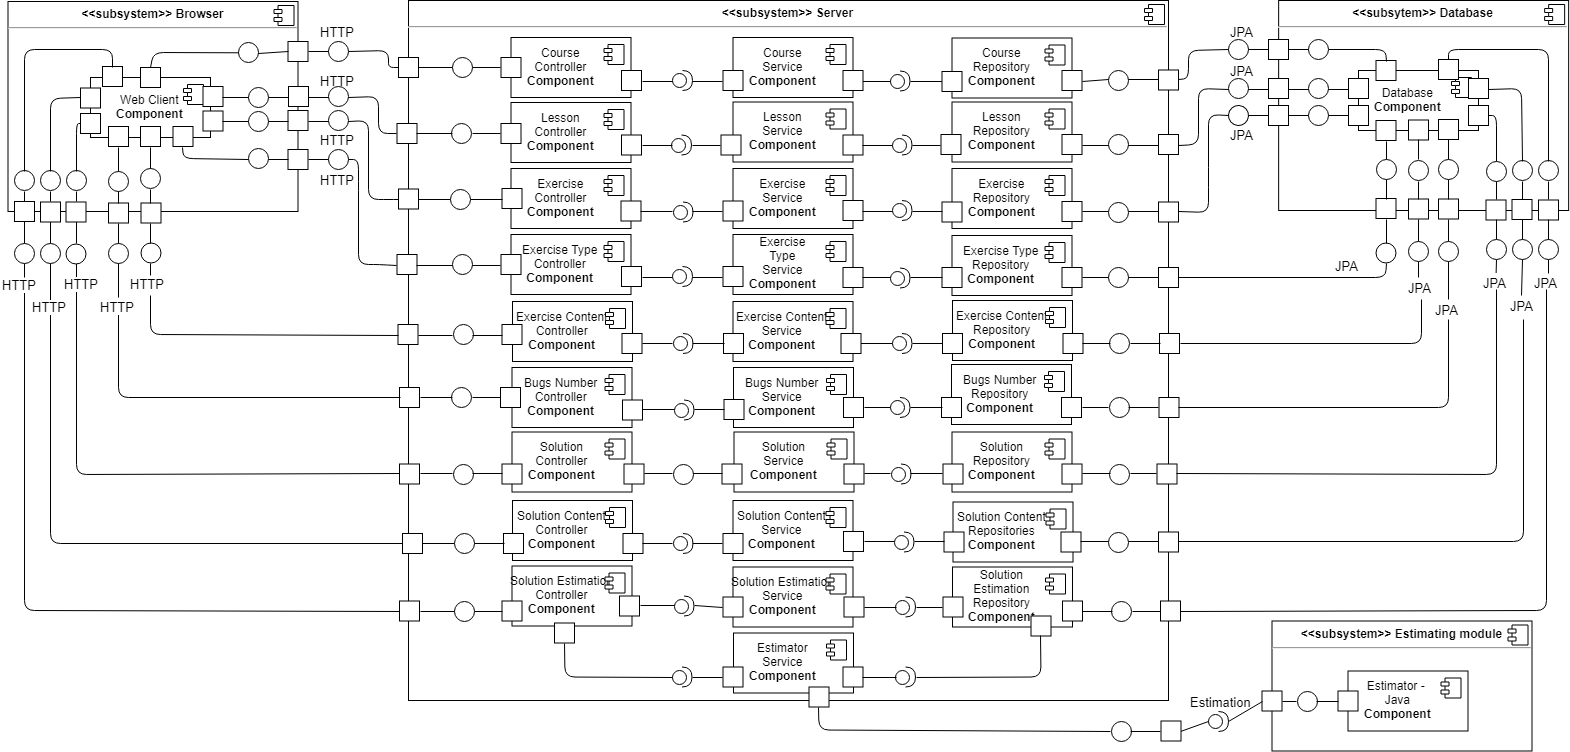
\includegraphics[width=0.9\textwidth, width=\linewidth]
        {images/component-diagram.png}}
    \caption{Component diagram}
    \label{fig:component-diagram}
    \end{sidewaysfigure}

    \section{User interface}
    This chapter is devoted to user interface concept.
    
        \subsection{Courses}
        The start page provides a list of the created courses and general information on them. With selecting one of the listed courses, the user may enter it. Also the user may manage the courses, e.g. create, edit or delete them, with the use of the button. This page leads to all of the application pages, and they contain ``Back'' button for easier navigation.
    
        When a course is entered, a new page contains an information about it. There is an expansion panel below with lessons and exercises they include. Every lesson and exercise may managed as well. Management includes editing, deleting, reordering and creation. The following sections are devoted to a detailed description of user interface for exercises creation, editing and solving.
    
        \subsection{Exercise creation and editing}
        Exercise creation and editing has the same structure, with difference in handing the user input and availability of initially defined values. The input fields change dynamically, depending on the exercise type of the exercise. It is possible to change exercise type without losing data the fields contain.
        
        Non-dynamic part contains fields for exercise title, description and exercise type selector. When an exercise type is chosen, the form changes and the corresponding editors appear. Every editor component have the same structure, and differ only with content and handling the user input.
        
        There are three types of editor. The first one is a source code editor, used for exercises of type \textit{Interactive Exercise} and \textit{Interactive Exercise with Files}. The second one is tests editor and used for exercises of type \textit{Black Box} and \textit{Black Box with Files}. And the last one is text editor, used for exercises of type \textit{Interactive Exercise with Files} and \textit{Black Box with Files}.
        
        The first type \textit{Theory} contains only description of the exercise. Exercise type \textit{Interactive Exercise} has editors for source code and tests, and exercise type \textit{Interactive Exercise with Files} has one more editor for text files.
        
        Application provides tool for convenient creation of two versions of source code, tests and text files. On exercise creation or update, there is an editor for a hidden version, and there is a select component below. The component contains two options for the shown version. The first option, ``the same'', is used when an exercise author wants the shown version to be the same a hidden. And the second option, ``custom'', is used to create or edit a different shown version, and an new editor element appears. Some of the exercise types requires only a hidden or shown version of source code or test, so there is no select component.
        
        The submit button is enabled as soon as the form input is valid. On submit, there appears a notification telling if the data were saved successfully. When cheating new exercise, there appears suggestion to create another one.
        
        \subsection{Exercise solving}
        When solving an exercise, its view is determined by its type. Every exercise types has view and functionality according to the concept, described in a section \ref{subsec:exercise-types} \nameref{subsec:exercise-types}.
        
        Every exercise contains a component for displaying a description. The description content is created with use of rich text editor. Editor components from the previous section are used for exercise solving as well.
        
        Every editor component is extended with version control component, as it required at the concept section \ref{subsec:version-control} \nameref{subsec:version-control}. It enables resetting the editor content and loading content from a submitted version.
        
        \subsection{Run output}
        On solving exercise of any type, except \textit{Thesis}, there is available a ``Run'' button for estimation a current result. When an exercise is submitted for the first time, an output area appears. During the estimation process, it contains ``Loading...'' message. When feedback is ready, it is printed out within the output. Feedback contains compilation and testing result for both public and private versions, and represented as percentage solving progress.
        
        Estimation runs two times for exercise types \textit{Interactive Exercise} and \textit{Interactive Exercise with Files}. First time for public version (running student's tests on his sources) and second time for private version (running teacher's tests on student's sources). The progress is represented as percentage and means how much tests were passed out of their total number.
        
        Testing result for exercise types \textit{Black Box} and \textit{Black Box with Files} contains only number of revealed mistakes and total number of them. The progress is represented as percentage, corresponding to the found mistakes number.
        
        \subsection{Exercise Toolbar}
        The pages for solving the exercises contain two equal toolbars, one on the top and second on the bottom of the page. They contain the mentioned ``Back'' button, navigation within the lesson exercises, and there is a flag representing the progress on the solving current exercise. Toolbar view changes dynamically on an exercise change.
    
    
    \section{Data structure}
    This section describes data model of the system for the resulting web application. It keeps account of created courses, lessons they contain, and exercises with used code and text files. Also it holds information about submitted solutions, used files and results. Data structure of the application is illustrated on diagram \ref{diagram:entity-rel-model}.

    The diagram shows a hierarchical structure of the courses, where each courses (\texttt{courses}) may contain several lessons (\texttt{lessons}), and each lesson contains exercises (\texttt{exercises}). These tables contain information about name, description and creation time. Lesson and exercises items have indexes, which defines in which order they should be solved.
    
    Every exercises has a type (\texttt{exercise types}). The ones, which have type \textit{Black Box (with Files)}, have a stored bugs number. Exercises have various types of content, each with different purpose, and they are subsets of \texttt{exercise content}.
    
    To store data about solutions, a table \texttt{solutions} was created for referencing on a corresponding exercise, and it is referenced from tables \texttt{solution estimation} and \texttt{solution content}. There are different types of solution files, and they are subsets of \texttt{solution content}.

    \begin{center}
    \begin{figure}[h]
    \begin{tikzpicture}
    
    \umlclass{courses}{
    	name\\
    	description\\
    	created\\
    }{}
    
    \umlclass[below=1 of courses]{lessons}{
    	name\\
    	description\\
    	created\\
    	index\\
    }{}
    \umlassoc[mult1=*,mult2=1]{lessons}{courses}
    
    \umlclass[right=2 of lessons]{solutions}{
        created\\
    }{}
    
    \umlclass[below=2 of solutions]{exercises}{
    	name\\
    	description\\
    	created\\
    	index\\
    	solved\\
    }{}
    \umlassoc[mult1=*,mult2=1]{exercises}{lessons}
    \umlassoc[mult1=*,mult2=1]{solutions}{exercises}
    
    \umlclass[below=2 of exercises]{exercise content}{
        filename\\
        content\\
    }{}
    \umlassoc[mult1=*,mult2=1]{exercise content}{exercises}
    
    \umlclass[left=2 of exercises]{exercise types}{
        name\\
        value\\
    }{}
    \umlassoc[mult1=*,mult2=1]{exercises}{exercise types}
    
    \umlclass[right=2 of exercises]{bugs number}{
        number\\
    }{}
    \umlassoc[mult1=*,mult2=1]{bugs number}{exercises}
    
    \umlclass[above=2 of solutions]{solution content}{
        filename\\
        content\\
    }{}
    \umlassoc[mult1=*,mult2=1]{solution content}{solutions}
    
    \umlclass[right=2 of solutions]{solution estimation}{
        estimation\\
        value\\
        solved\\
        created\\
    }{}
    \umlassoc[mult1=*,mult2=1]{solution estimation}{solutions}
    
    
    \umlclass[left=2 of exercise content]{private source}{}{}
    \umlinherit{private source}{exercise content}
    
    \umlclass[below=2 of private source]{private test}{}{}
    \umlinherit{private test}{exercise content}
    
    \umlclass[right=1 of private test]{private file}{}{}
    \umlinherit{private file}{exercise content}
    
    \umlclass[right=2 of exercise content]{public source}{}{}
    \umlinherit{public source}{exercise content}
    
    \umlclass[below=2 of public source]{public test}{}{}
    \umlinherit{public test}{exercise content}
    
    \umlclass[left=1 of public test]{public file}{}{}
    \umlinherit{public file}{exercise content}
    
    
    \umlclass[above=2 of solution content]{solution test}{}{}
    \umlinherit{solution test}{solution content}
    
    \umlclass[left=1 of solution test]{solution source}{}{}
    \umlinherit{solution source}{solution content}
    
    \umlclass[right=1 of solution test]{solution file}{}{}
    \umlinherit{solution file}{solution content}
    
    \end{tikzpicture}
    \caption{Entity relationship model}
    \label{model}
    \end{figure}
    \end{center}
    

    \section{Use cases}
    The users of the application are divided into two groups, teachers and students. In fact, the application does not separate these groups, so any user can be an author and a solver. Use case diagram illustrates how these two groups interact with the system.
    
    \begin{sidewaysfigure}
    \centerline{
        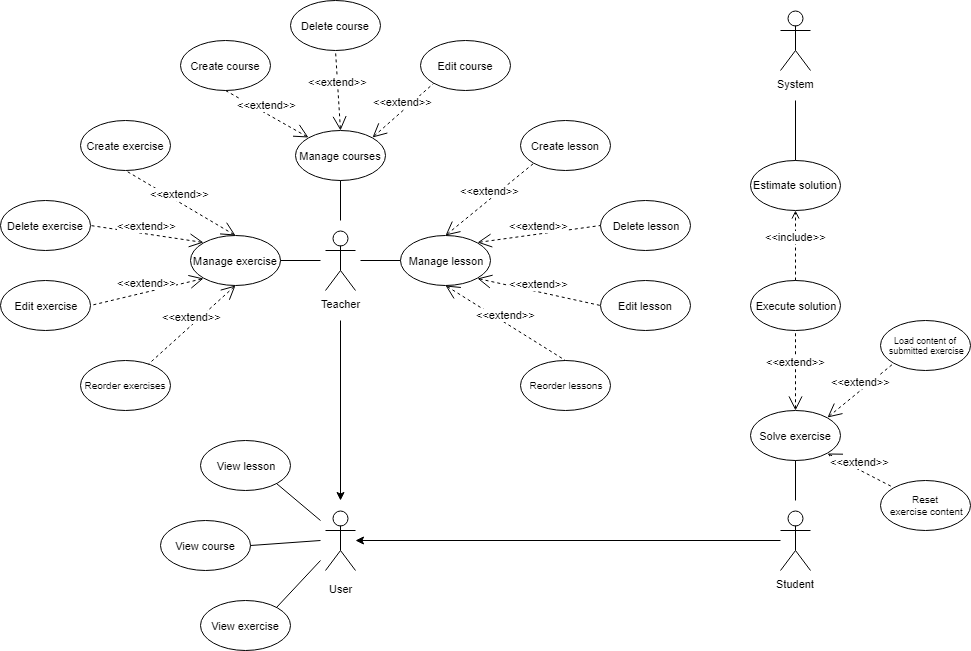
\includegraphics[width=\textwidth]
        {images/use-case.png}}
    \caption{Use case diagram}
    \label{fig:use-case}
    \end{sidewaysfigure}

    \section{Technical requirements}
    \label{sec:tech-requirements}
    This section is devoted to the requirements for the resulting web application and their purpose.
        
        \subsection{Security}
        \label{subsec:security}
        Another important requirement concerns about security issues and elimination of the potential risks.
        
        Running the programs, written by teachers and students, on the server brings risks for the system. Running the program would be isolated, and its would have limited access to the rest of the system. It may be aimed with use of a form of a software vitalisation, a \textit{virtual sandbox}.
        
        Another web application security risk is \textit{Cross-Site Scripting} (XSS), which allows malicious code to be added to a web page via user input, e.g. form submissions, and used in it \cite[A7-Cross-Site Scripting (XSS)]{owasp_xss}. To prevent this, the input would be sanitised: rather than accept or reject input, another option is to change the user input into an acceptable format \cite[Sanitize]{owasp_sanitize}. Such an attack may be used in text editor for an exercise description.
